\section{Verbindungsmanagement}
\label{subsec:verbindungsmanagement}

Das Verbindungsmanagement ist ein essentieller Bestandteil des Protokolls, da es die Grundlage für die Kommunikation zwischen den Teilnehmern bildet. Es ist dafür verantwortlich, dass die Nachrichtenübertragung zwischen den Teilnehmern funktioniert. Dazu gehört der Verbindungsaufbau, die Nachrichtenübertragung und der Verbindungsabbau, welche im Folgenden detailliert beschrieben werden.

\subsection{Verbindungsaufbau}
\label{label:verbindungsaufbau}

Bei der Herstellung einer Verbindung zwischen zwei Teilnehmern sind die IP-Adresse und der Port des Zielgeräts entscheidend. Der Port ist durch die Definition in Abschnitt \ref{subsec:identifikation_von_teilnehmern} bereits festgelegt und damit bekannt. Sobald die IP-Adresse des Ziels über Kademlia ermittelt wurden, wird versucht, eine direkte Verbindung herzustellen. Grundsätzlich gilt, dass eine direkte Verbindung vor allen anderen Verbindungsarten bevorzugt wird. Im Falle einer erfolglosen Suche im Kademlia-Netzwerk, gilt der Teilnehmer zu diesem Zeitpunkt als nicht erreichbar bzw. \textit{offline}. Wird allerdings eine IP-Adresse ermittelt, wird ein UDP-Paket an diese gesendet. Es wird erwartet, dass das Ziel innerhalb eines festgelegten Zeitfensters antwortet. Wenn eine Antwort innerhalb dieses Zeitrahmens eingeht, wird die Kommunikation über diesen direkten Weg aufgebaut und ein Austausch von Nachrichten kann beginnen. Falls keine Antwort eintrifft, gibt es das zweite Verfahren, um eine Verbindung herzustellen: das \textit{Interactive Connectivity Establishment} (kurz: \textit{ICE}) Protokoll. Wenn also die direkte Verbindung scheitert, tritt das ICE-Protokoll in Kraft.
Ursprünglich war die Idee, dass bei einer fehlgeschlagenen direkten Verbindung ein Relay-Server mit dem TURN-Protokoll verwendet werden soll. Doch aus nachfolgendem Zitat ist zu entnehmen, dass TURN nicht die beste Lösung ist, da nicht definiert ist, wie die \textit{relayed transport address}, mit deren Hilfe die Kommunikation über den Relay-Server aufgebaut werden soll, an die Teilnehmer kommuniziert werden soll.

\begin{quote}
    \textit{A client using TURN must have some way to communicate the relayed transport address to its
    peers and to learn each peer's IP address and port (more precisely, each peer's server-reflexive
    transport address; see Section 3). How this is done is out of the scope of the TURN protocol. One
    way this might be done is for the client and peers to exchange email messages.} \parencite[S. 7]{rfc8656_TURN}
\end{quote}


\noindent Deshalb wurde sich, wenn die direkte Verbindung nicht funktioniert, für die Verwendung des ICE-Protokolls entschieden. ICE ist ein Protokoll, das die Verbindungseinrichtung zwischen zwei Geräten ermöglicht, die sich hinter NATs (Network Address Translation) befinden \parencite[S. 6-7]{rfc8445_ICE}. Es ist ein Protokoll, das in der Lage ist, sich an sich ändernde Netzwerkbedingungen anzupassen und verschiedene Arten von Verbindungen zu unterstützen, wie beispielsweise direkte Verbindungen, Verbindungen über STUN (Session Traversal Utilities for NAT) oder Verbindungen über TURN (Traversal Using Relays around NAT) \parencite[S. 1]{rfc8445_ICE}. 

Um eine Verbindung zwischen zwei Geräten aufzubauen, durchläuft ICE drei Phasen: die Sammlung und der Austausch von Verbindungsadressen, die Konnektivitätsprüfung und die Auswahl der am besten geeigneten Verbindungsadresse für die Kommunikation \parencite{rfc8445_ICE}.

Die erste Phase beinhaltet das Sammeln verschiedener potenzieller Verbindungsadressen (auch \textit{Kandidatenadressen} genannt \parencite[S. 8]{rfc8445_ICE}), die für eine zuverlässige Kommunikation benötigt werden, insbesondere wenn einer oder beide Teilnehmer sich hinter NATs befinden. Zuallererst werden die lokalen oder \textit{Host}-Adressen der beteiligten Geräte berücksichtigt. Diese Adressen repräsentieren die standardmäßigen IP-Adressen und Ports der Geräte innerhalb ihres lokalen Netzwerks. Sie dienen als potenzielle direkte Verbindungswege zwischen den Geräten, falls sie sich im gleichen Netzwerk oder Subnetz befinden.
Zusätzlich zu den lokalen Adressen werden reflexive Adressen über STUN (Session Traversal Utilities for NAT) ermittelt. STUN ermöglicht es einem Gerät, seine eigene externe IP-Adresse und den entsprechenden Port zu identifizieren, wie sie von einem NAT-Gerät reflektiert werden \parencite[S. 4]{rfc8489_STUN}. Diese reflexiven Adressen stellen die externe Sichtbarkeit des Geräts aus der Perspektive des NAT-Geräts dar und helfen bei der Umgehung von NAT-Beschränkungen für den direkten Verbindungsaufbau. Sollte es jedoch aufgrund von restriktiven NAT-Konfigurationen nicht möglich sein, eine direkte Verbindung aufzubauen, kommen Relay-Adressen durch TURN (Traversal Using Relays around NAT) ins Spiel.
Durch TURN werden Relay-Server genutzt, um den Datenverkehr zwischen den Geräten zu vermitteln \parencite[S. 10-11]{rfc8656_TURN}. Diese Weiterleitungsadressen dienen als alternative Verbindungsmethode, indem sie den Datenverkehr über den Relay-Server leiten und so die Hindernisse von restriktiven NATs umgehen.
Die kombinierte Nutzung dieser verschiedenen Arten von potenziellen Verbindungsadressen – von lokalen, reflexiven bis hin zu Relay-Adressen – ermöglicht eine Vielzahl von Optionen für die Verbindungseinrichtung zwischen den Geräten. Diese Vielfalt an Adressen gewährleistet, dass selbst in komplexen Netzwerkszenarien wie NATs oder Firewalls verschiedene Wege für eine zuverlässige Kommunikation vorhanden sind.

Nachdem alle potenziellen Verbindungsadressen gesammelt wurden, werden sie an den anderen Teilnehmer gesendet. Dieser Prozess wird als \textit{Kandidatenaustausch} bezeichnet und erfolgt unter Verwendung eines Signaling Servers. Aus der Definition von ICE geht nicht hervor, wie die Verbindungsadressen zwischen den Teilnehmern (in ICE als \textit{Agents} bezeichnet) ausgetauscht werden sollen. Wie aus dem nachstehenden Zitat zu verstehen ist, nimmt das Protokoll an, dass die Agents dazu in der Lage sind, doch wie genau das geschehen soll, ist nicht definiert \Parencite{rfc8445_ICE}.

\begin{quote}
    \textit{In a typical ICE deployment, there are two endpoints (ICE agents)
    that want to communicate. [...]. ICE assumes that the agents are able to
    establish a signaling connection between each other.} \parencite[S. 7]{rfc8445_ICE}
\end{quote}

\noindent Eine eigene Definition für den Austausch der Verbindungsadressen zwischen den Teilnehmern über einen Signaling Server zu erstellen, ginge über den Umfang dieser Arbeit hinaus. Ein Ansatz wäre, dass der Server die Benutzernamen der Teilnehmer kennt oder die Existenz des Benutzernamens eventuell via Smart Contract prüfen kann (siehe \ref{subsec:contract_registrierung} \textit{\nameref{subsec:contract_registrierung}}), und somit die Verbindungsadressen der anfragenden Teilnehmer anhand der Benutzernamen an die jeweiligen Teilnehmer sendet. Abbildung \ref{fig:signaling_server} stellt ein Beispiel eines Ablaufs des Kandidatenaustauschs über einen Signaling Server mit Hilfe eines Sequenzdiagramms dar:

\begin{center}
    \captionsetup{type=figure}
    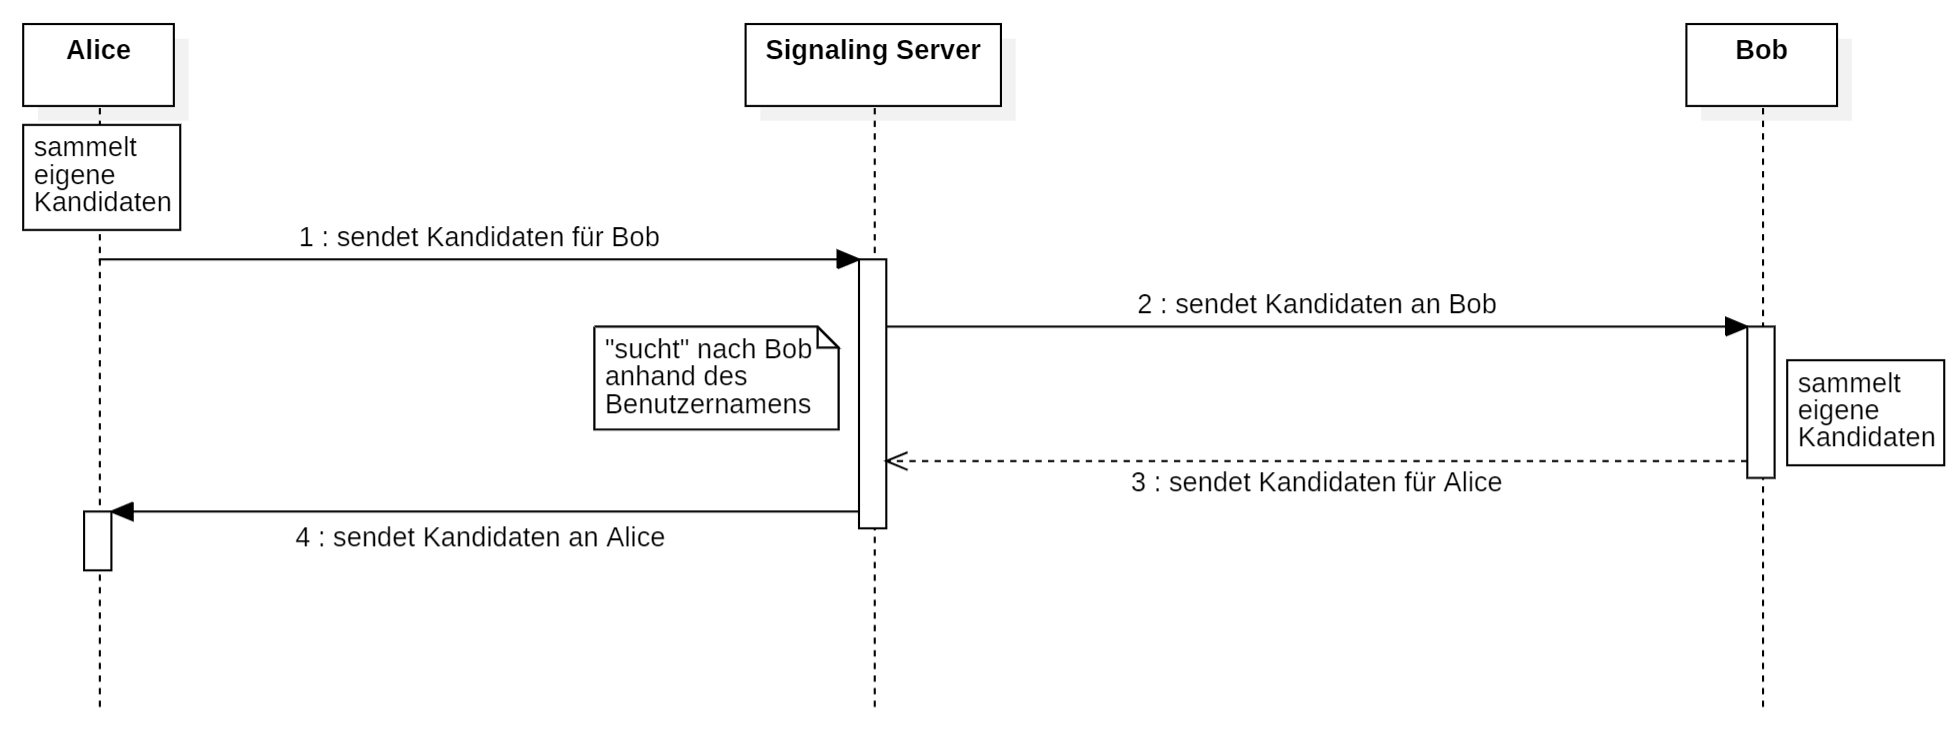
\includegraphics[width=1.0\linewidth]{images/signaling_sequence.png}
    \captionof{figure}{Kandidatenaustausch über einen Signaling Server}
    \label{fig:signaling_server}
\end{center}

\noindent Alice möchte eine Verbindung zu Bob aufbauen. Dazu sendet sie eine Verfügbarkeitsabfrage an den Signaling Server. Zusätzlich sendet sie ihre Kandidatenadressen mit, die sie zuvor gesammelt hat. Der Signaling Server erhält die Kandidatenadressen von Alice und prüft, ob Bob verfügbar ist. Wenn dies der Fall ist, sendet der Signaling Server die Kandidatenadressen von Alice an Bob. Bob speichert die Kandidatenadressen von Alice und sendet seine eigenen Kandidatenadressen an den Signaling Server. Der Signaling Server leitet diese dann an Alice weiter. Sollte Bob allerdings nicht verfügbar sein, sendet der Signaling Server eine Fehlermeldung an Alice. 

Man könnte nun argumentieren, dass Kademlia durch die Verwendung von ICE überflüssig wird, da auch ICE die lokale IP-Adresse und den Port des Empfängers ermitteln kann und somit eine direkte Verbindung aufgebaut werden könnte. Doch Kademlia wird bewusst weiterhin verwendet, da es die Auslastung des Signaling Servers so gering wie möglich hält, indem der erste Versuch des Verbindungsaufbaus immer über Kademlia erfolgt. Außerdem ist immer noch das Ziel, möglichst ohne jegliche Server auszukommen. Aus diesem Grund wird das ICE-Protokoll nur dann verwendet, wenn der Verbindungsaufbau über Kademlia fehlschlägt. Durch das Beibehalten dieser Struktur wird die Anzahl der Verbindungsversuche über den Signaling Server minimiert. Je nach Teilnehmeranzahl kann die Anzahl der Verbindungsversuche über den Signaling Server sehr hoch sein, was zu einer hohen Auslastung des Servers führen kann.

In Phase zwei werden Konnektivitätsprüfungen durchgeführt. Diese Prüfungen dienen dazu, die Eignung und Zuverlässigkeit der gesammelten Verbindungswege zwischen den Geräten zu bewerten, um die bestmögliche Verbindung für eine erfolgreiche Kommunikation zu identifizieren. Die Reihenfolge der Konnektivitätsprüfungen wird durch einen Prioritätsalgorithmus bestimmt, der die Verbindungsadressen nach ihrer Priorität ordnet. Dies wird vom Initiator der Verbindung durchgeführt, der die Verbindungsadressen der anderen Teilnehmer erhält. Aus der Dokumentation von ICE geht hervor, dass die Priorität einer Verbindungsadresse durch die folgende Formel berechnet wird \parencite[S. 22]{rfc8445_ICE}:

\begin{equation}
    \label{eq:ice_priority}
    \text{priority} = \text{2}^{24} \cdot \text{(type preference)} + \text{2}^{8} \cdot \text{(local preference)} + \text{2}^{0} \cdot \text{(256 - component ID)}
\end{equation}

\noindent Jeder Kandidat hat eine Priorität, die durch die Formel \ref{eq:ice_priority} berechnet wird. Die Priorität wird durch die drei Parameter in der Formel bestimmt: Typpräferenz, lokale Präferenz und Komponenten-ID. Die Typpräferenz ist ein Parameter, der die Art der Verbindungsadresse angibt, und dessen Wert sich zwischen $0$ und $126$ befinden muss. Es gibt, wie bereits in Phase eins aufgezeigt, drei verschiedene Typen von Verbindungsadressen: Host-Adressen, Peer-reflexive Adressen und Relay-Adressen. Die Werte für die Typpräferenz, die in der Dokumentation von ICE für die Berechnung der Priorität empfohlen werden, sind die folgenden: $126$ für Host-Adressen, $100$ für Peer-reflexive Adressen und $0$ für Relay-Adressen. Wichtig ist, dass der Wert $0$ für Relay-Adressen nicht bedeutet, dass Relay-Adressen nicht verwendet werden sollten, sondern dass sie die niedrigste Priorität haben. Für das Protokoll dieser Arbeit werden diese Werte übernommen. Für die lokalen Präferenzen wird ein Wert von $65535$ empfohlen, um die Verwendung von lokalen Adressen zu priorisieren. Auch dieser Wert wird übernommen. Der dritte und letzte Wert der Formel ist die Komponenten-ID, die dazu dient, verschiedene Datenströme oder Komponenten innerhalb eines einzelnen Kandidaten zu unterscheiden. Das bedeutet, dass ein Kandidat mehrere Komponenten haben kann, die jeweils eine eigene Komponenten-ID haben. Dadurch können beispielweise Bild-Daten, Audio-Daten und Text-Daten innerhalb eines einzelnen Kandidaten über verschiedene Komponenten gesendet werden. Da in dem Protokoll dieser Arbeit nur ein Datenstrom verwendet wird - und zwar Text - wird der Komponenten-ID der Wert $1$ zugewiesen. Zur Veranschaulichung wird die Berechnung der Priorität für die drei verschiedenen Arten von Adressen anhand der vergebenen Werte in der Formel \ref{eq:ice_priority} dargestellt. Für die Berechnung der Priorität für Host-Adressen sieht die Formel wie folgt aus:

\begin{equation}
    \label{eq:ice_priority_protocol_host}
    \text{priority} = \text{2}^{24} \cdot \text{(126)} + \text{2}^{8} \cdot \text{(65535)} + \text{2}^{0} \cdot \text{(256 - 1)}
\end{equation}

\noindent Die Priorität für Peer-reflexive Adressen lautet wie folgt:

\begin{equation}
    \label{eq:ice_priority_protocol_reflexive}
    \text{priority} = \text{2}^{24} \cdot \text{(100)} + \text{2}^{8} \cdot \text{(65535)} + \text{2}^{0} \cdot \text{(256 - 1)}
\end{equation}

\noindent Die Priorität für Relay-Adressen lautet wie folgt:

\begin{equation}
    \label{eq:ice_priority_protocol_relay}
    \text{priority} = \text{2}^{24} \cdot \text{(0)} + \text{2}^{8} \cdot \text{(65535)} + \text{2}^{0} \cdot \text{(256 - 1)}
\end{equation}

\noindent Wenn alle Kandidaten ihre Priorität erhalten haben, werden sie nach ihrer Priorität sortiert und die Konnektivitätsprüfung beginnt. Dieser Prozess beinhaltet den Versuch, Verbindungen aufzubauen und Datenverkehr über verschiedene potenzielle Wege zu senden und zu empfangen. Durch das Senden von Probe-Paketen über jede potenzielle Verbindungsadresse wird geprüft, ob eine Verbindung aufgebaut werden konnte. Dabei werden die drei verschiedenen Arten von Adressen (lokale, reflexive und Relay-Adressen) verwendet, um verschiedene Möglichkeiten zu testen, wie die Geräte miteinander kommunizieren können. 

Die Probe-Pakete werden über UDP (kurz für: \textit{User Datagram Protocol}) gesendet, da es ein verbindungsloses Protokoll ist und somit vor dem Senden keine Verbindung aufgebaut werden muss \parencite[S. 1]{rfc768_UDP}. Dies ermöglicht es, die Erreichbarkeit der Verbindungsadressen zu testen, ohne eine Verbindung aufzubauen. Die Probe-Pakete werden an die Verbindungsadressen gesendet und die Antwort wird überwacht. Wenn eine Antwort empfangen wird, wird die Verbindungsadresse als erreichbar angesehen. Wenn keine Antwort empfangen wird, wird die Verbindungsadresse als nicht erreichbar angesehen. Um die Stabilität der Verbindungsadressen zu testen, werden in regelmäßigen Abständen Probe-Pakete gesendet. Wenn die Probe-Pakete über einen längeren Zeitraum nicht beantwortet werden, wird die Verbindungsadresse als nicht stabil angesehen. 

Mit dem Abschluss der Konnektivitätsprüfungen beginnt die dritte und letzte Phase. Mit den Ergebnissen werden Kandidaten-Paare gebildet, die die Verbindungsadressen der beiden Geräte enthalten. Während dieses Schritts werden die gesammelten Kandidaten (lokale IP-Adressen, Ports und durch STUN oder TURN-Server erhaltene Reflexionen) in verschiedenen Konstellationen kombiniert. Jede dieser Kombinationen bildet ein Paar, das als möglicher Kommunikationsweg zwischen den Geräten dienen könnte. Die gebildeten Paare werden auf Redundanz kontrolliert und dann nach ihrer Priorität sortiert, die aus den einzelnen Prioritäten der Kandidaten berechnet wird. Aus dieser Reihenfolge wird dann die sogenannte \textit{Checkliste} erstellt, die die Paare in der Reihenfolge ihrer Priorität enthält. Auch die Kandidaten-Paare erhalten mit Hilfe einer Formel eine Priorität, die in der Dokumentation von ICE auf Seite 31 definiert ist \parencite[S. 31]{rfc8445_ICE}. Anschließend  wird damit begonnen, eine Verbindung über das Paar mit der höchsten Priorität aufzubauen. Wenn die Verbindung erfolgreich aufgebaut werden kann, wird die Kommunikation über dieses Paar fortgesetzt. Wenn die Verbindung nicht erfolgreich aufgebaut werden kann, wird das Paar mit der nächsthöheren Priorität ausgewählt und der Prozess wird wiederholt. Dieser Prozess wird fortgesetzt, bis eine Verbindung erfolgreich aufgebaut werden kann. Wenn keine Verbindung aufgebaut werden kann, wird die Kommunikation über das Paar mit der höchsten Priorität fortgesetzt, das eine Verbindung über den Relay-Server verwendet. Die folgende Abbildung \ref{fig:ice_sequence} stellt den Ablauf des ICE-Prozesses bildlich, mit Hilfe eines Sequenzdiagramms, dar:

\begin{center}
    \captionsetup{type=figure}
    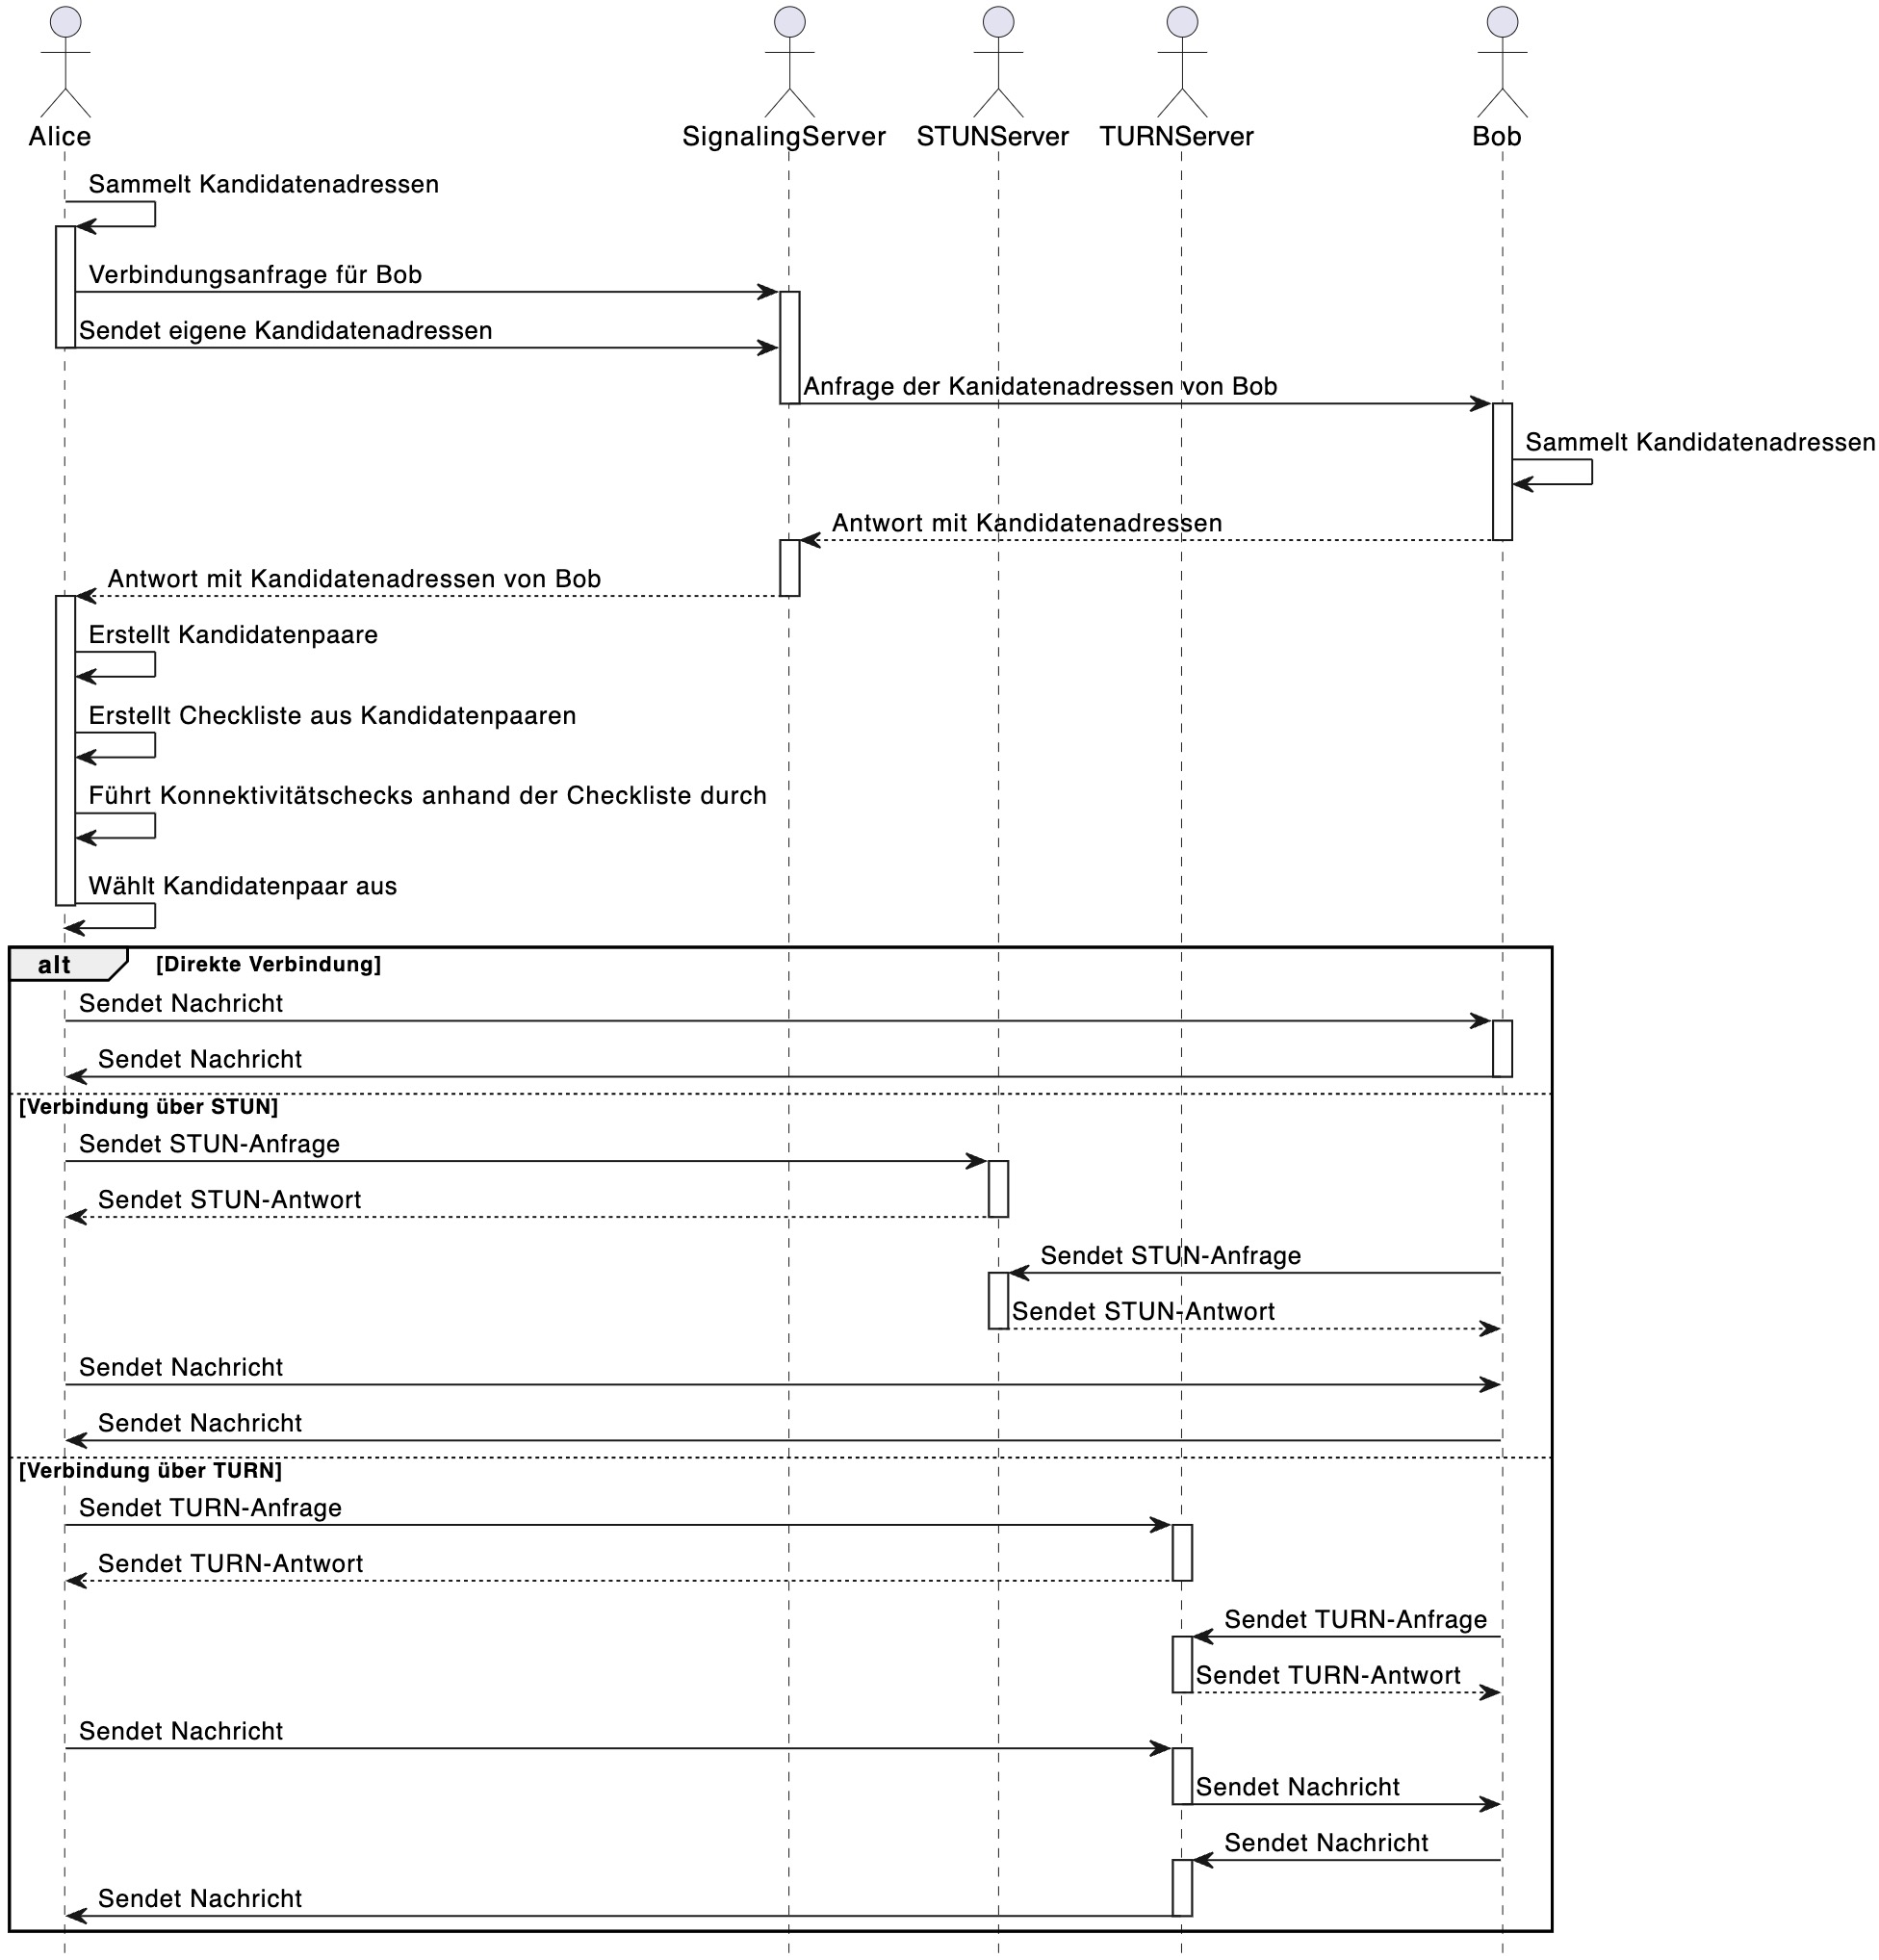
\includegraphics[width=1.0\linewidth]{images/ice_corrected.jpg}
    \captionof{figure}{ICE-Prozess}
    \label{fig:ice_sequence}
\end{center}

\noindent Ein großer Vorteil von ICE ist die Flexibilität, die es ermöglicht, sich an sich ändernde Netzwerkbedingungen anzupassen. Falls sich während der Kommunikation Netzwerkparameter ändern - beispielsweise durch einen Wechsel zwischen Wi-Fi und Mobilfunknetzwerken - kann ICE dynamisch neue Kandidatenadressen identifizieren und die Verbindungen anpassen, ohne die laufende Kommunikation zu unterbrechen.

\subsection{Nachrichtenübertragung}

Wenn die am besten geeignete Verbindungsadresse eine lokale Adresse ist, wird eine direkte Verbindung zwischen den Geräten aufgebaut. Wenn die am besten geeignete Verbindungsadresse eine reflexive Adresse ist, wird eine direkte Verbindung zwischen den Geräten aufgebaut, indem die reflexive Adresse als Zieladresse verwendet wird. Wenn wiederum die am besten geeignete Verbindungsadresse eine Relay-Adresse ist, wird eine Verbindung über den Relay-Server aufgebaut, indem die Relay-Adresse als Zieladresse verwendet wird. Der Nachrichtenaustausch erfolgt über die ausgewählte Verbindungsadresse. Wobei hier mit \textit{Verbindung aufbauen} gemeint ist, dass die Nachrichten über die Verbindungsadresse gesendet und empfangen werden können. Aus Sicht der Transportschicht wird durch die Verwendung von UDP keine Verbindung aufgebaut, denn UDP ist, wie bereits erwähnt, ein verbindungsloses Protokoll. Das bedeutet, dass keine Verbindung aufgebaut werden muss, um die Nachrichten zu senden und zu empfangen. Aus Applikationssicht wird jedoch eine Verbindung aufgebaut, da die Nachrichten zwischen den Teilnehmern ausgetauscht werden können.

Ein Nachteil bei der Verwendung von UDP ist, dass die Nachrichten nicht zuverlässig zugestellt werden. Das bedeutet, dass Nachrichten verloren gehen können, ohne dass der Absender oder Empfänger davon erfährt. Das Transportprotokoll TCP (Transmission Control Protocol) hingegen ist zuverlässig, da es eine Verbindung aufbaut und sicherstellt, dass die Nachrichten erfolgreich zugestellt werden \parencite[S. 36]{rfc9293_TCP}. Im Falle von Paketverlusten ist auf der gleichen Seite definiert, dass TCP in der Lage ist, die verlorenen Pakete zu erkennen und erneut zu senden.

Doch eine mögliche Verwendung von TCP hat auch Nachteile: ein Nachteil ist, dass es eine Verbindung aufbauen muss, bevor die Nachrichten gesendet werden können. Dies kann zu einer höheren Latenz führen. Ein weiterer Nachteil ist, dass die Verbindung aufrechterhalten werden muss, um die Nachrichten zu senden und zu empfangen. Dies führt zu einem höheren Ressourcenverbrauch, da die Verbindung aufrechterhalten werden muss, auch wenn keine Nachrichten gesendet werden. Auch bei NATs hat TCP Nachteile. NATs schließen die Verbindungen nach einer gewissen Zeit, wenn keine Daten übertragen werden. Dies kann dazu führen, dass die Verbindung geschlossen werden, bevor die Nachrichten gesendet werden können. 
Ein überzeugendes Argument für die Verwendung von UDP liegt in seiner Effizienz durch den geringeren Overhead im Vergleich zu TCP. Dank des schlankeren Headers werden weniger Daten übertragen, was besonders in Instant Messaging-Szenarien, in denen kleine Nachrichten häufig versendet werden, zu einer effizienteren Nutzung der Netzwerkressourcen und zu schnelleren Übertragungen führt. UDP bietet zudem den Vorteil der Unabhängigkeit in Bezug auf die Reihenfolge der übermittelten Pakete. Im Gegensatz zu TCP, das die korrekte Reihenfolge sicherstellt, überlässt UDP diese Aufgabe der Anwendungsschicht. In Instant-Messaging-Anwendungen, in denen die Reihenfolge der Nachrichten möglicherweise weniger kritisch ist, ermöglicht dies eine flexiblere und potenziell schnellere Übertragung von Nachrichten. Die geringere Verbindungsetablierungszeit von UDP ist ein weiterer Pluspunkt. Da UDP ein verbindungsloses Protokoll ist, entfällt der zeitliche Aufwand für das Auf- und Abbauen von Verbindungen. Dies ist besonders vorteilhaft in Umgebungen mit häufigen Verbindungswechseln, wie sie bei Instant-Messaging mittels Peer-to-Peer auftreten können. Die Minimierung der Latenzzeit trägt dazu bei, Nachrichten schneller bereitzustellen \parencites{rfc768_UDP}{rfc9293_TCP}. 
Aus diesen Gründen wurde UDP als Transportprotokoll für die Nachrichtenübertragung gewählt.


\subsection{Verbindungsabbau}

Durch die Verwendung von UDP ist es nicht möglich, eine Verbindung aktiv zu schließen. Deshalb wird die Verbindung durch einen Timeout geschlossen, der nach einer gewissen Zeit abläuft, wenn keine Nachrichten mehr gesendet werden.